% !TeX program = xelatex
% !TeX spellcheck = en_US
% $Id: example.tex,v 1.1.1.1 2003/11/12 19:21:55 vverdult Exp $
%
%\documentclass[generic]{tudposter} % Template without wind turbines
\documentclass[wind]{tudposter} % Template with wind turbines

\usepackage{tikz}
\usetikzlibrary{arrows,shadows,calc,positioning}
\usepackage{multicol} % use multiple columns
\usepackage{graphicx}
\usepackage{xcolor,pgf}
\usepackage{caption}
\usepackage{enumitem}
\columnsep=100pt      % spacing between the columns of text
\columnseprule=0pt    % width of separating line between the columns

\setlength{\parindent}{0pt}
\setlength{\parskip}{2ex}

\usepackage{fontspec}
\begin{document}

\LARGE % select sans serif font and enlarge fonts

% Create the title and the personal section
\maketitle{A title about my research project that spans two lines}{images/profilephoto.jpg}{Bart Doekemeijer}{b.m.doekemeijer@tudelft.nl}{linkedin.com/in/bartdoekemeijer}

% Create core content
\setmainfont[Ligatures=TeX,Path=./fonts/,BoldItalicFont=calibrii.ttf,BoldFont=calibri.ttf,ItalicFont=calibrili.ttf]{calibril.ttf}
\begin{multicols}{2} % use two columns

%%%%%%%%%%%%%%%%%

\section{Summary}
Lorem ipsum dolor sit amet, \textcolor{orange}{consectetur} adipiscing elit. Etiam iaculis faucibus hendrerit. Maecenas ut auctor arcu. Sed iaculis efficitur \textcolor{tudblue}{augue sed auctor}. Vestibulum erat risus, dictum non eleifend eget, lacinia et odio. Donec eget finibus orci, sit amet condimentum risus. Ut mi risus, ultrices ut tincidunt posuere, ultricies vel ex. Etiam quis nisl vel dolor tempus auctor \textcolor{orange}{quis vel urna}. Donec sapien tortor, ornare ut arcu vitae, egestas volutpat ex. Aliquam scelerisque rhoncus quam in scelerisque. In nulla nisl, dictum vitae pharetra at, tempor \textcolor{tudblue}{vitae mauris}.\\

%%% FIGURE
\begin{minipage}{\linewidth}
	\centering
	\vspace{5mm}
	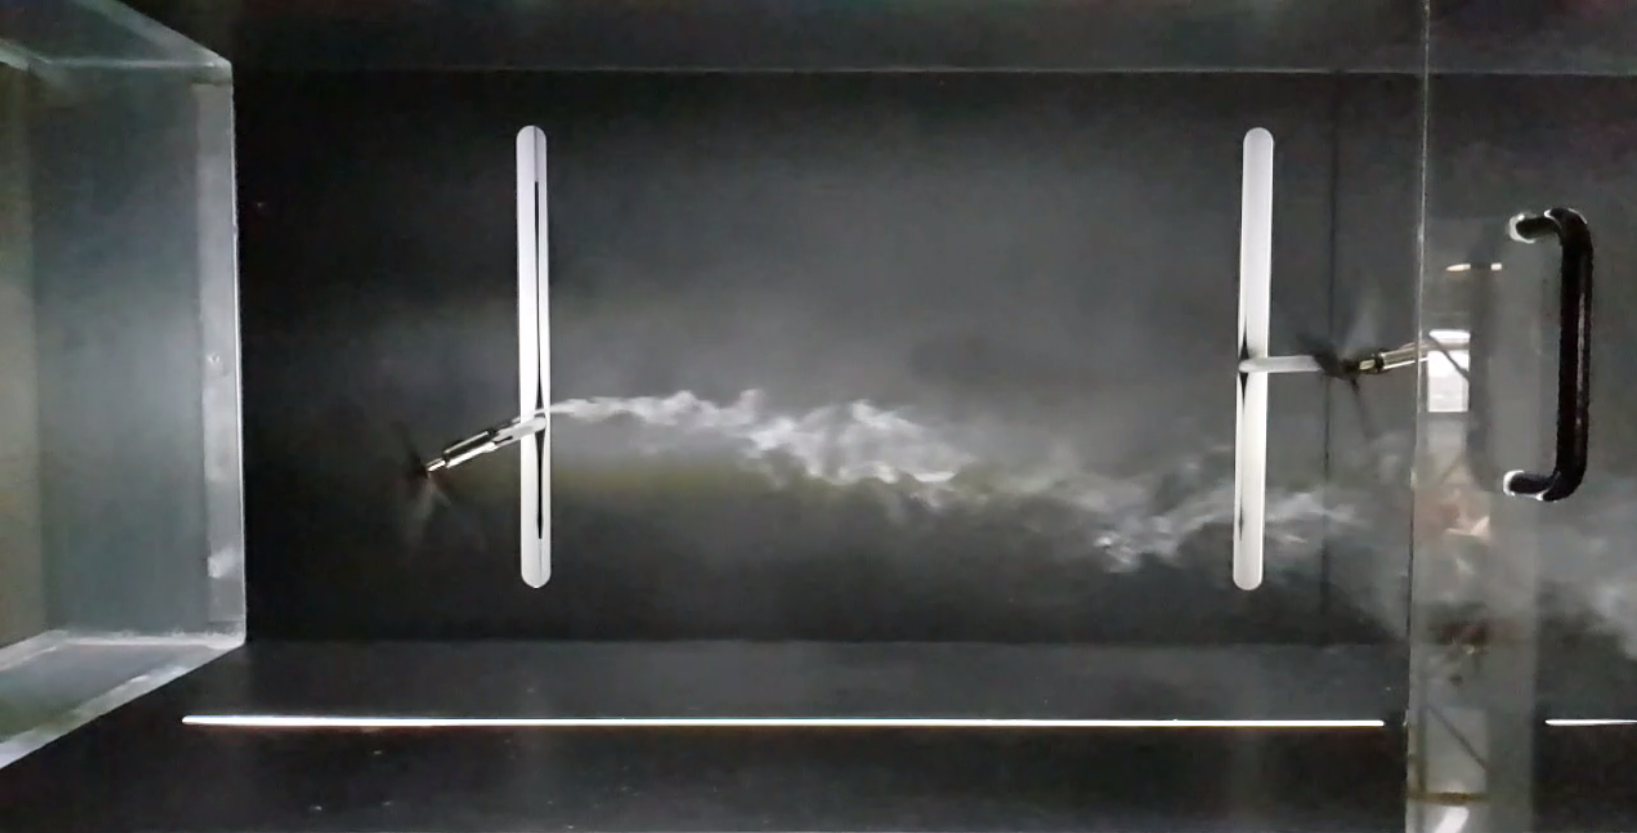
\includegraphics[width=\linewidth]{images/windtunnel.png}
	{Figure: Wake steering demonstrated in our wind tunnel} % Optional caption
	\vspace{1cm}
\end{minipage}
%% END OF FIGURE

% Section
\section{Motivation}	
Donec nec ante neque. Etiam consequat, tortor id mattis gravida, justo sapien fermentum lorem, eu efficitur purus diam et est. Curabitur pharetra lacus magna, sit amet cursus libero porta eu. 
\begin{itemize}[noitemsep,leftmargin=3cm,labelsep=7mm,label=\textcolor{tudblue}{$\bullet$}]
	\item Suspendisse sollicitudin,
	\item diam ut euismod blandit,
	\item nulla tortor viverra diam,
	\item eget lacinia ex felis eu metus.
\end{itemize} 
Duis pharetra justo vitae porta sollicitudin. Nunc lobortis mi velit, eu mollis libero consectetur in. Duis ac molestie dolor, ut condimentum lorem.

Nunc placerat enim nisl, in fermentum tortor tempus at. Aenean vitae metus consequat, molestie velit vel, condimentum lectus. Praesent tempus magna vitae ornare ornare. Nam accumsan blandit mauris, sit amet accumsan massa placerat id.

% Section
\section{Case study}
Suspendisse ultrices velit lobortis nisl fringilla, quis porttitor leo posuere. Nam id vehicula ante. Suspendisse tempus tincidunt sagittis. Aliquam erat volutpat. In finibus, sapien a venenatis iaculis, quam elit pellentesque ante, non dignissim nisl velit ut orci.

%%% FIGURE
\begin{minipage}{\linewidth}
	\centering
	\vspace{5mm}
	\begin{minipage}[b]{.55\linewidth}
	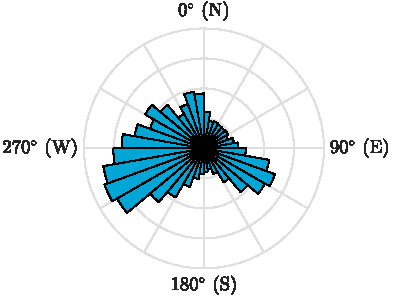
\includegraphics[width=\textwidth]{images/histogram_wd.pdf}
	\end{minipage}
	\begin{minipage}[b]{.42\linewidth}
	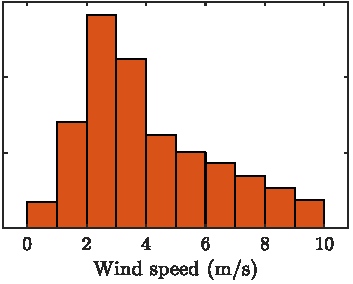
\includegraphics[width=\textwidth]{images/histogram_ws.pdf}	
	\end{minipage}
	\vspace{2cm}
\end{minipage}
%% END OF FIGURE

Pellentesque pharetra molestie eros. Ut aliquam commodo tempor. Sed hendrerit sem nibh, id malesuada nisi faucibus egestas. Morbi egestas eget orci id placerat. In nec lectus rhoncus, imperdiet dolor quis, ultricies elit. Duis dignissim egestas mi, dignissim lacinia ipsum dapibus eget.\\


\begin{minipage}[h!]{\linewidth}
	\centering
	{Table: Benchmark results}\\
	\vspace{1cm}
	\begin{tabular}{| m{8cm}  |  m{11cm}  | m{11cm}  |}\hline
		\textbf{Criteria} & \textbf{Old method} & \textbf{New method} \\\hline
		criteria 1 & score & score \\\hline
		criteria 2 & score & score \\\hline
		criteria 3 & score & score \\\hline
		criteria 4 & score & score \\\hline
	\end{tabular}
	\vspace{2cm}
\end{minipage}

Lorem ipsum dolor sit amet, consectetur adipiscing elit. Phasellus sit amet eros consequat, eleifend erat a, tempus velit. Quisque eu sem urna. Lorem ipsum dolor sit amet, consectetur adipiscing elit. Phasellus sit amet eros consequat, eleifend erat a, tempus velit. Quisque eu sem urna.\\
\end{multicols}

% Bottom banner with information about the software and a QR code. This could also be a personal website or something linked to your research. You can create your own QR codes at https://www.qr-code-generator.com.
\vspace{22mm}
\begin{center}
	\begin{minipage}[b]{66mm}
		
\includegraphics[width=\linewidth]{images/qrcode.png} 
	\end{minipage}%
\begin{minipage}[b]{52cm}
\fbox{\begin{tikzpicture}
\node[preaction={fill=white,fill opacity=0.75}] (c) { \begin{minipage}{50cm} \Large{\textit{The software tools presented are created by the Data-Driven Controls group of the TU Delft. Our software tools are developed, maintained and shared on our publicly available Github repository. You can find our tools at  \textcolor{tudblue}{https://github.com/TUDelft-DataDrivenControl}.}} \end{minipage}};
\end{tikzpicture}}
\vspace{5mm}
\end{minipage}
\end{center}

%\begin{center}
%\begin{tabular}{m{7cm} m{54cm}}
%
\includegraphics[width=7cm,trim=0 4cm 0 0]{images/qrcode.png} & \fbox{\begin{minipage}{\linewidth} \vspace{5mm} 
%\centering
%\begin{minipage}{0.97\linewidth} % Add horizontal spacing between box and text
%\Large{\textit{The software tools presented are created by the Data-Driven Controls group of the TU Delft. Our software tools are developed, maintained and shared on our publicly available Github repository. You can find our tools at  \textcolor{tudblue}{https://github.com/TUDelft-DataDrivenControl}.}}\end{minipage}
%\vspace{5mm}
%\end{minipage}}
%\end{tabular}
%\end{center}

\end{document}